\chapter{Results}
\label{chap:results}

This chapter reports the empirical evidence produced by the pipeline
defined in Chapter~\ref{chp:experiments_and_framework}. Every number in
this chapter is traceable to a script and an artefact in the
repository; every claim is qualified by its confidence interval or its
inherent uncertainty. The chapter is organised so that the reader
encounters the evidence in the same order in which the hypotheses of
Section~\ref{sec:data_aware_hypotheses} depend on it.

Section~\ref{sec:results_eventlog_char} reports the descriptive
characteristics of the training and testing partitions produced by the
split of Section~\ref{sec:train_test_split}.
Section~\ref{sec:results_process_discovery} reports the discovered
Petri net and its conformance on both partitions (RQ2).
Section~\ref{sec:results_arrival_process} reports the temporal
structure of the arrival process (H1).
Section~\ref{sec:results_holdout_fidelity} reports the held-out
Monte-Carlo fidelity of the three ProSiT configurations
(RQ1, H2, H3). Section~\ref{sec:results_per_activity} decomposes the
fidelity by activity to identify where each configuration wins or
loses. Section~\ref{sec:results_resource_capacities} reports the
discovered resource capacities and their limits.
Section~\ref{sec:results_percentile_sens} reports the sensitivity of
the transition-baseline choice (RQ3).
Section~\ref{sec:results_scenarios} reports the two what-if scenarios
(H4). Section~\ref{sec:results_summary} consolidates the empirical
findings against the hypotheses.

%%%%%%%%%%%%%%%%%%%%%%%%%%%%%%%%%%%%%%%%%%%%%%%%%%%%%%%%%%%%%%
\section{Event Log Characteristics on the Held-Out Split}
\label{sec:results_eventlog_char}
%%%%%%%%%%%%%%%%%%%%%%%%%%%%%%%%%%%%%%%%%%%%%%%%%%%%%%%%%%%%%%

The train/test split of Section~\ref{sec:train_test_split} yields a
temporally ordered partition of the 89,458 cases. Cases with earliest
event timestamp $\le\text{2026-04-20 18:14}$ form the training log
(71,566 cases, 221,559 events, cases spanning
\text{2026-03-02 05:25} through the cutoff). Cases with earliest event
timestamp $>\text{2026-04-20 18:14}$ form the testing log (17,892
cases, 55,864 events). No events are dropped for missing timestamps.
Table~\ref{tab:activity_counts_split} lists the per-activity counts in
both partitions.

\begin{table}[h]
\centering
\caption{Activity counts on the train and test partitions.}
\label{tab:activity_counts_split}
\begin{tabular}{lrrr}
\toprule
\textbf{Activity} & \textbf{Train} & \textbf{Test} & \textbf{Total} \\
\midrule
Gate In       & 71,566 & 17,892 & 89,458 \\
Gate Out      & 71,566 & 17,892 & 89,458 \\
RMG\_receive  & 30,656 & 7,678  & 38,334 \\
RMG\_delivery & 14,010 & 3,514  & 17,524 \\
RMG\_mixed    & 10,816 & 2,706  & 13,522 \\
LL\_delivery  & 7,678  & 1,911  & 9,589  \\
HO2\_delivery & 5,351  & 1,338  & 6,689  \\
HO2\_receive  & 3,807  & 955    & 4,762  \\
LL\_mixed     & 3,571  & 880    & 4,451  \\
HO2\_mixed    & 1,810  & 444    & 2,254  \\
LL\_receive   & 728    & 182    & 910    \\
\bottomrule
\end{tabular}
\end{table}

The per-activity distribution on the test partition is proportional to
the training partition to within 1--3\,\% for the four RMG-related
activities and within 5\,\% for the low-frequency activities
(\texttt{LL\_receive}, \texttt{HO2\_mixed}). No activity is missing from
the test partition. The split therefore does not introduce
class-imbalance artefacts that would confound the fidelity comparison
in Section~\ref{sec:results_holdout_fidelity}.

%%%%%%%%%%%%%%%%%%%%%%%%%%%%%%%%%%%%%%%%%%%%%%%%%%%%%%%%%%%%%%
\section{Process Discovery and Held-Out Conformance}
\label{sec:results_process_discovery}
%%%%%%%%%%%%%%%%%%%%%%%%%%%%%%%%%%%%%%%%%%%%%%%%%%%%%%%%%%%%%%

The Petri net is discovered from the training partition with the
inductive miner as described in
Section~\ref{sec:process_discovery_methodology}. Table~\ref{tab:conformance_train_test}
reports the four conformance metrics on both partitions.

\begin{table}[h]
\centering
\caption{Petri-net conformance on train and test.}
\label{tab:conformance_train_test}
\begin{tabular}{lrr}
\toprule
\textbf{Metric} & \textbf{Train} & \textbf{Test} \\
\midrule
Fitness (token-based replay)     & 1.000 & 1.000 \\
Precision (token-based replay)   & 0.904 & 0.872 \\
Generalisation                   & 0.974 & 0.949 \\
Simplicity                       & 0.652 & 0.652 \\
\bottomrule
\end{tabular}
\end{table}

Fitness of $1.000$ on the training log is expected: the inductive miner
is fitness-preserving by construction. Fitness of $1.000$ on the
held-out testing log is not automatic: it demonstrates that the
control-flow structure discovered on the first 80\,\% of the cases
replays every case in the last 20\,\% without token deficit. Precision
drops from 0.904 to 0.872 (a relative reduction of 3.5\,\%) and
generalisation from 0.974 to 0.949 (a relative reduction of 2.6\,\%).
Simplicity depends only on the Petri-net structure and is identical
across partitions.

The size of the discovered Petri net is 42 places, 59 transitions and
128 arcs. The training log contains 134 trace variants; the top-3
variants account for 67.5\,\% of all cases and the top-20 variants for
98.7\,\%. The remaining variants correspond to low-frequency
operational deviations
(e.g.\ \texttt{Gate In}$\to$\texttt{HO2\_mixed}$\to$\texttt{LL\_delivery}$\to$\texttt{Gate Out}
with 41 cases).

Figure~\ref{fig:petri_net} shows the discovered Petri net enriched with
token-replay frequency; edge labels report the number of tokens that
crossed the corresponding transition during replay on the training log.
The visualisation makes the process structure explicit: after
\texttt{Gate In} the flow branches at a first exclusive choice
between RMG, LL and HO2 handling; the three handling families each
carry an internal exclusive choice between \texttt{receive},
\texttt{delivery} and \texttt{mixed} sub-activities; the flow
re-converges before \texttt{Gate Out}. The relative arc thickness
mirrors the activity counts of Table~\ref{tab:activity_counts_split}:
the RMG family dominates ($\approx 63\,\%$ of yard activities), the LL
family follows ($\approx 21\,\%$) and the HO2 family is the least
frequent ($\approx 16\,\%$). No unreachable transitions or dead places
appear in the net.

\begin{figure}[htbp]
\centering
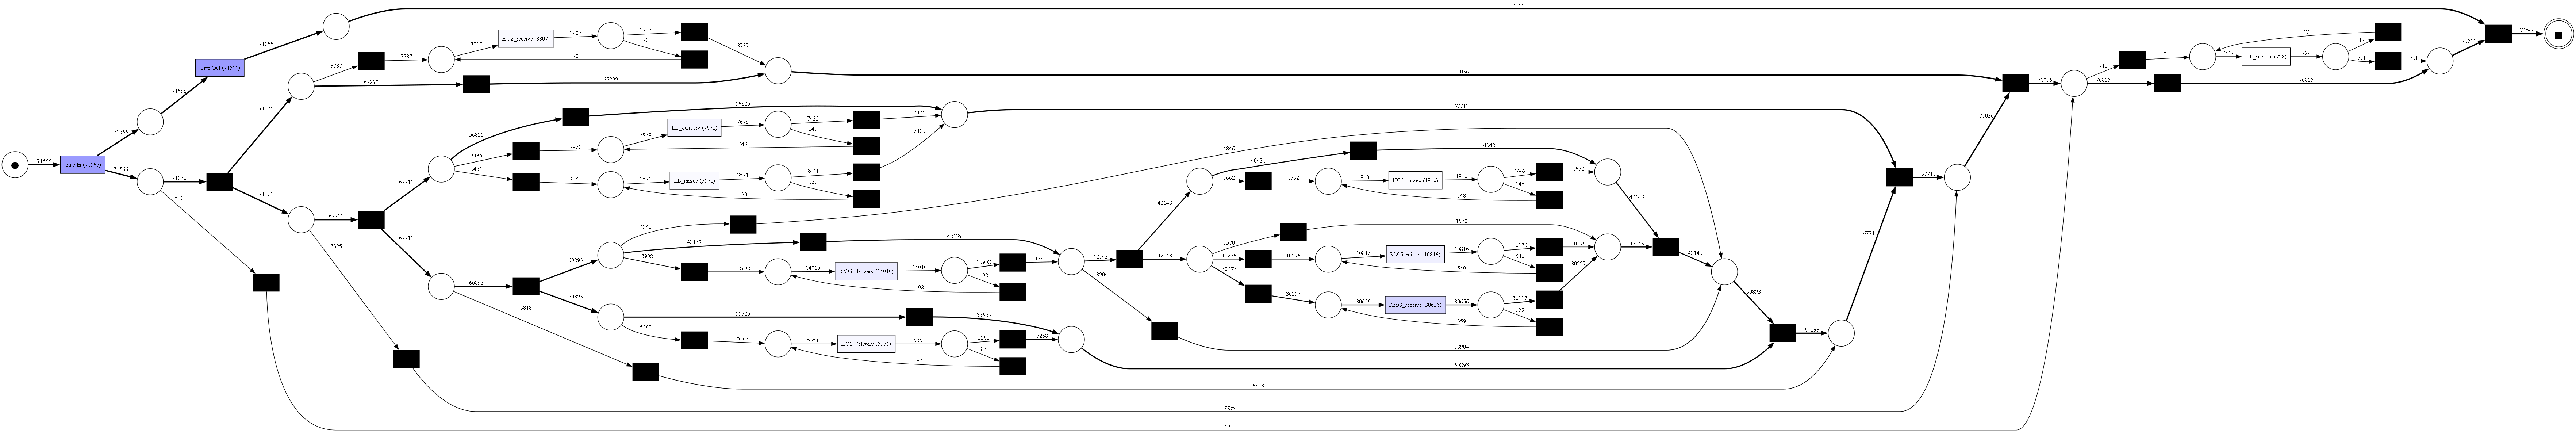
\includegraphics[width=0.95\textwidth]{figures/discovery/petri_net_frequency.png}
\caption{Discovered Petri net with token-replay frequency on the
training log (71,566 cases, 221,559 events). Transition labels report
the number of replayed tokens. The visualisation is produced by
\texttt{pm4py.visualization.petri\_net.visualizer} in the
\texttt{FREQUENCY} variant.}
\label{fig:petri_net}
\end{figure}

Figure~\ref{fig:dfg_freq} shows the directly-follows graph of the
training log. This is a complementary view to the Petri net:
whereas the Petri net encodes the concurrency and exclusive choice
structure inferred by the inductive miner, the DFG shows the raw
handover statistics between activities. The dominant paths
\texttt{Gate~In}$\to$\texttt{RMG\_receive}$\to$\texttt{Gate~Out},
\texttt{Gate~In}$\to$\texttt{RMG\_delivery}$\to$\texttt{Gate~Out} and
\texttt{Gate~In}$\to$\texttt{RMG\_mixed}$\to$\texttt{Gate~Out}
carry 30k, 14k and 11k cases respectively.

\begin{figure}[htbp]
\centering
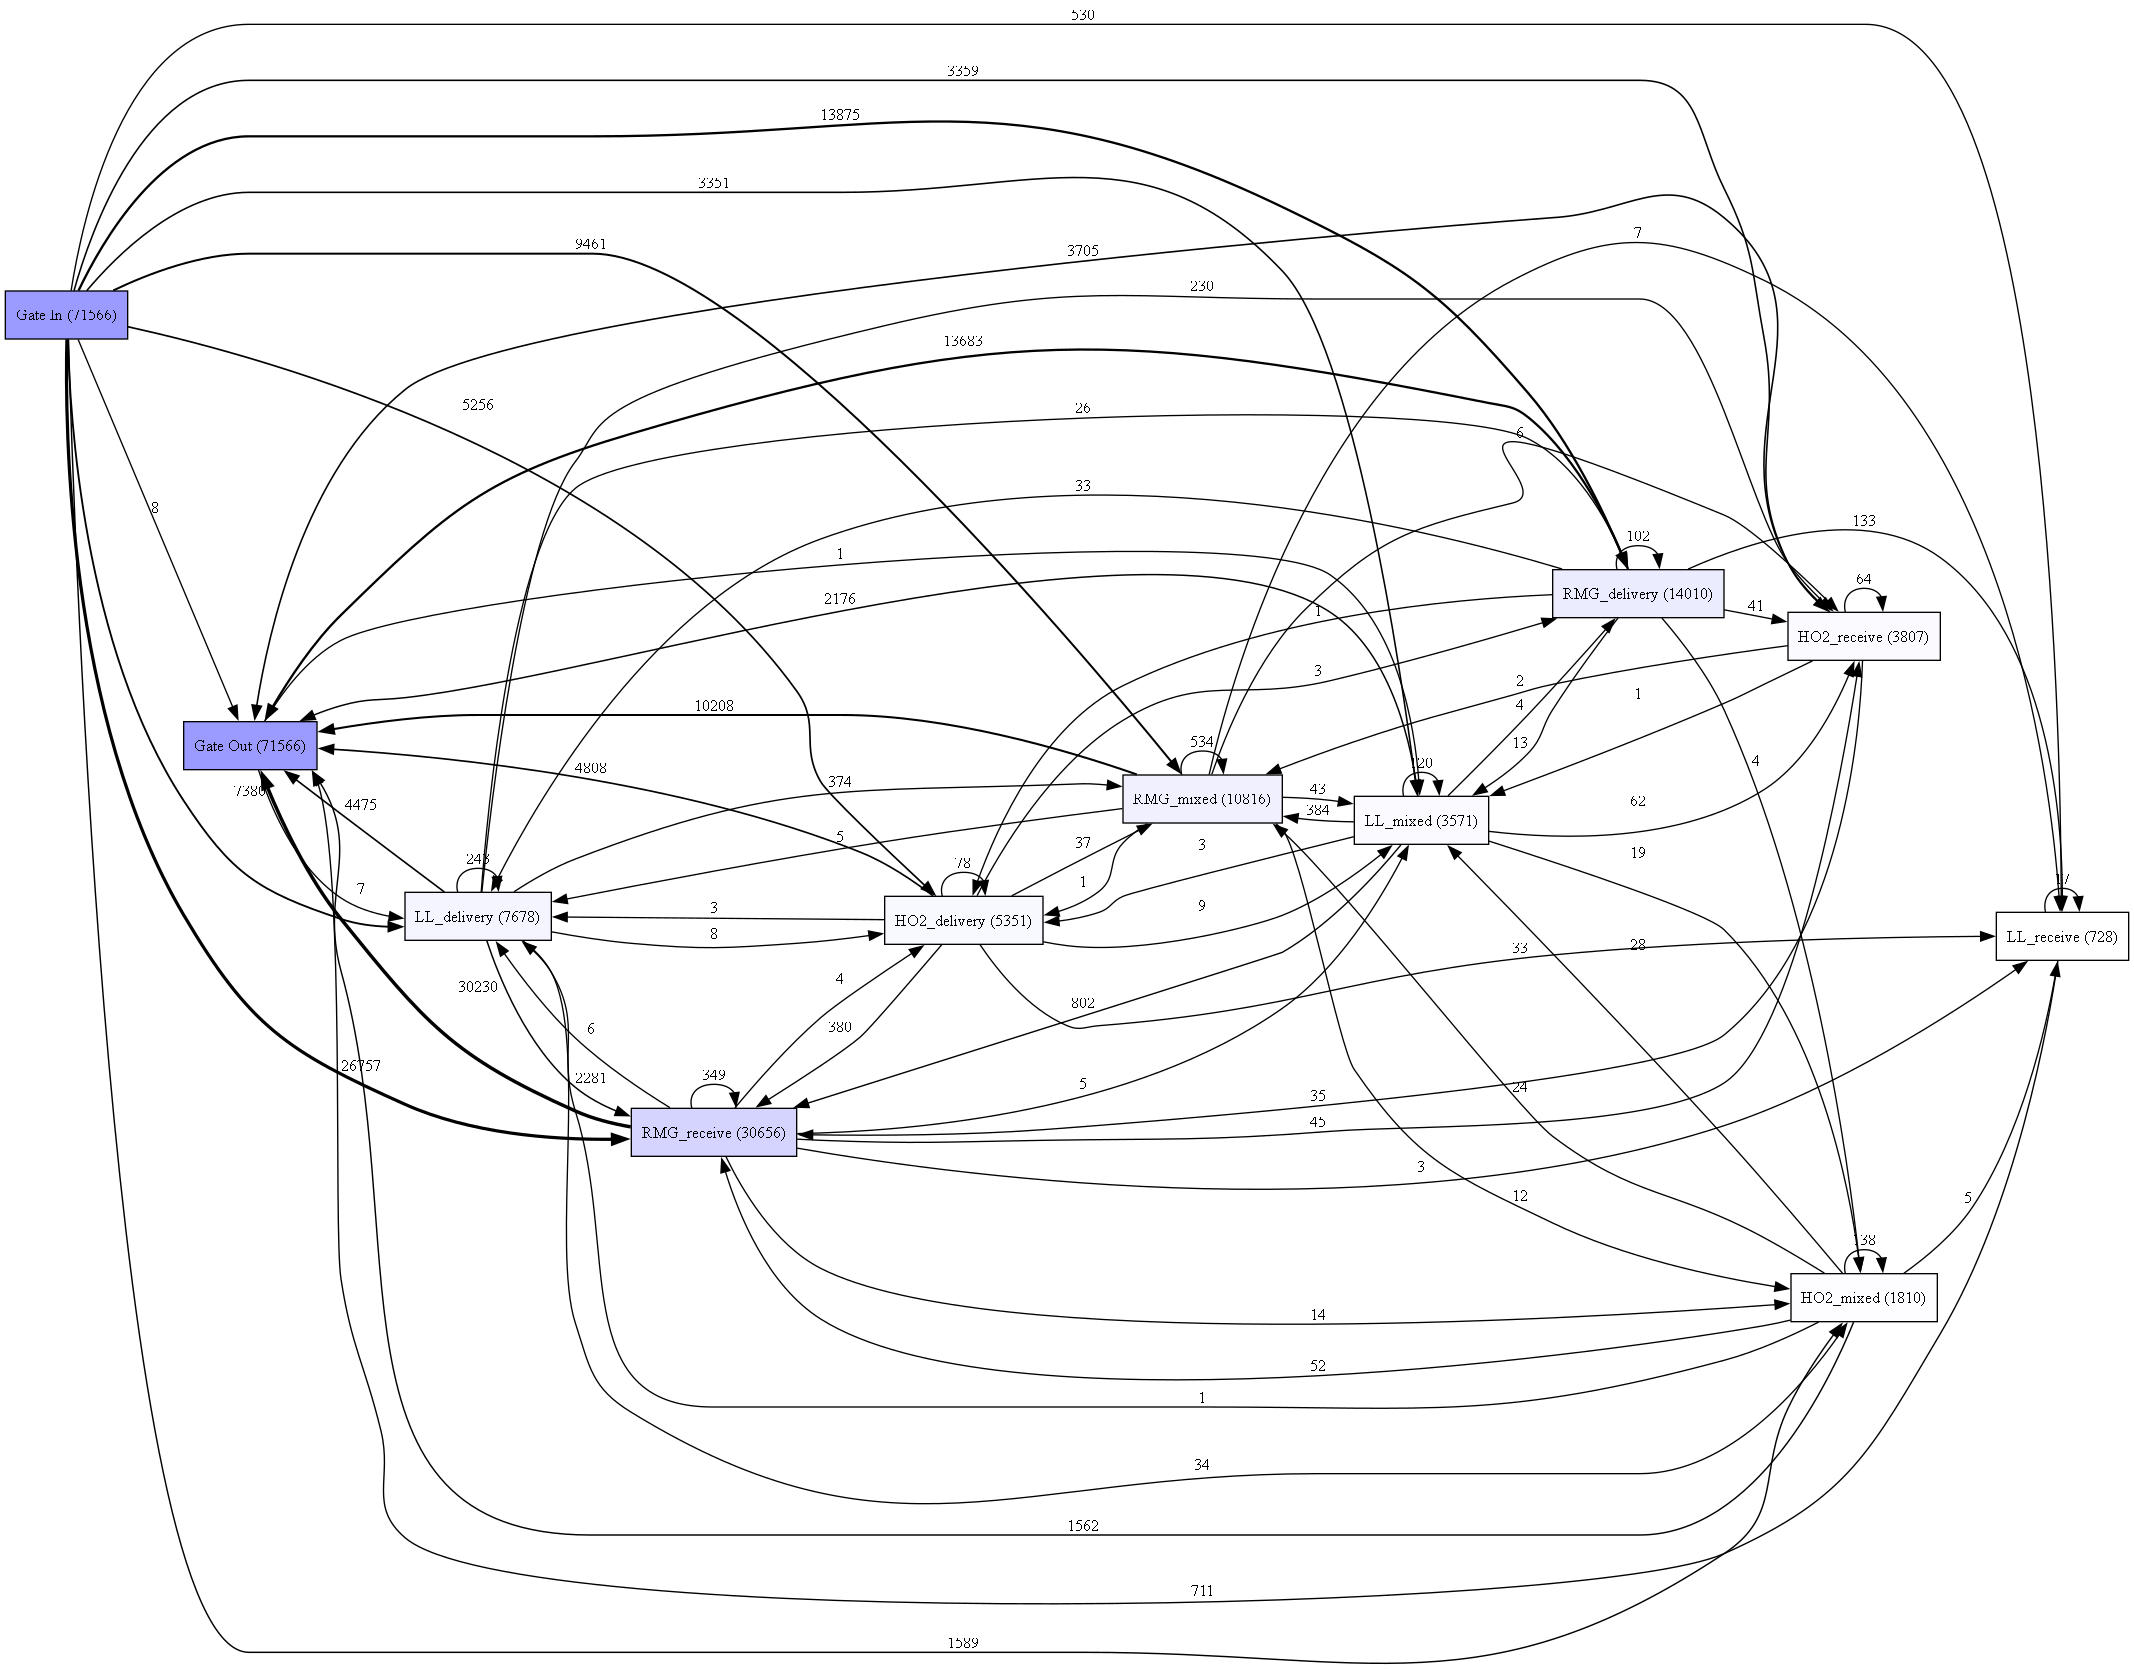
\includegraphics[width=0.85\textwidth]{figures/discovery/dfg_frequency.png}
\caption{Directly-follows graph of the training log with edge
frequencies. Complementary to the Petri net in
Figure~\ref{fig:petri_net}: shows raw handover statistics between
activities.}
\label{fig:dfg_freq}
\end{figure}

Figure~\ref{fig:variants_top20} confirms the concentration of behaviour
in a small number of variants. The top 20 trace variants cover 98.7\,\%
of the 71,566 training cases; the tail of 114 additional variants
accounts for only 908 cases and consists mainly of visits that combine
two yard families in a single visit (e.g.\ HO2 receive followed by an
RMG delivery). The event log is therefore structurally regular: the
Petri net of Figure~\ref{fig:petri_net} is a compact representation of
the observed control flow, not a coarse simplification of a highly
variable process.

\begin{figure}[htbp]
\centering
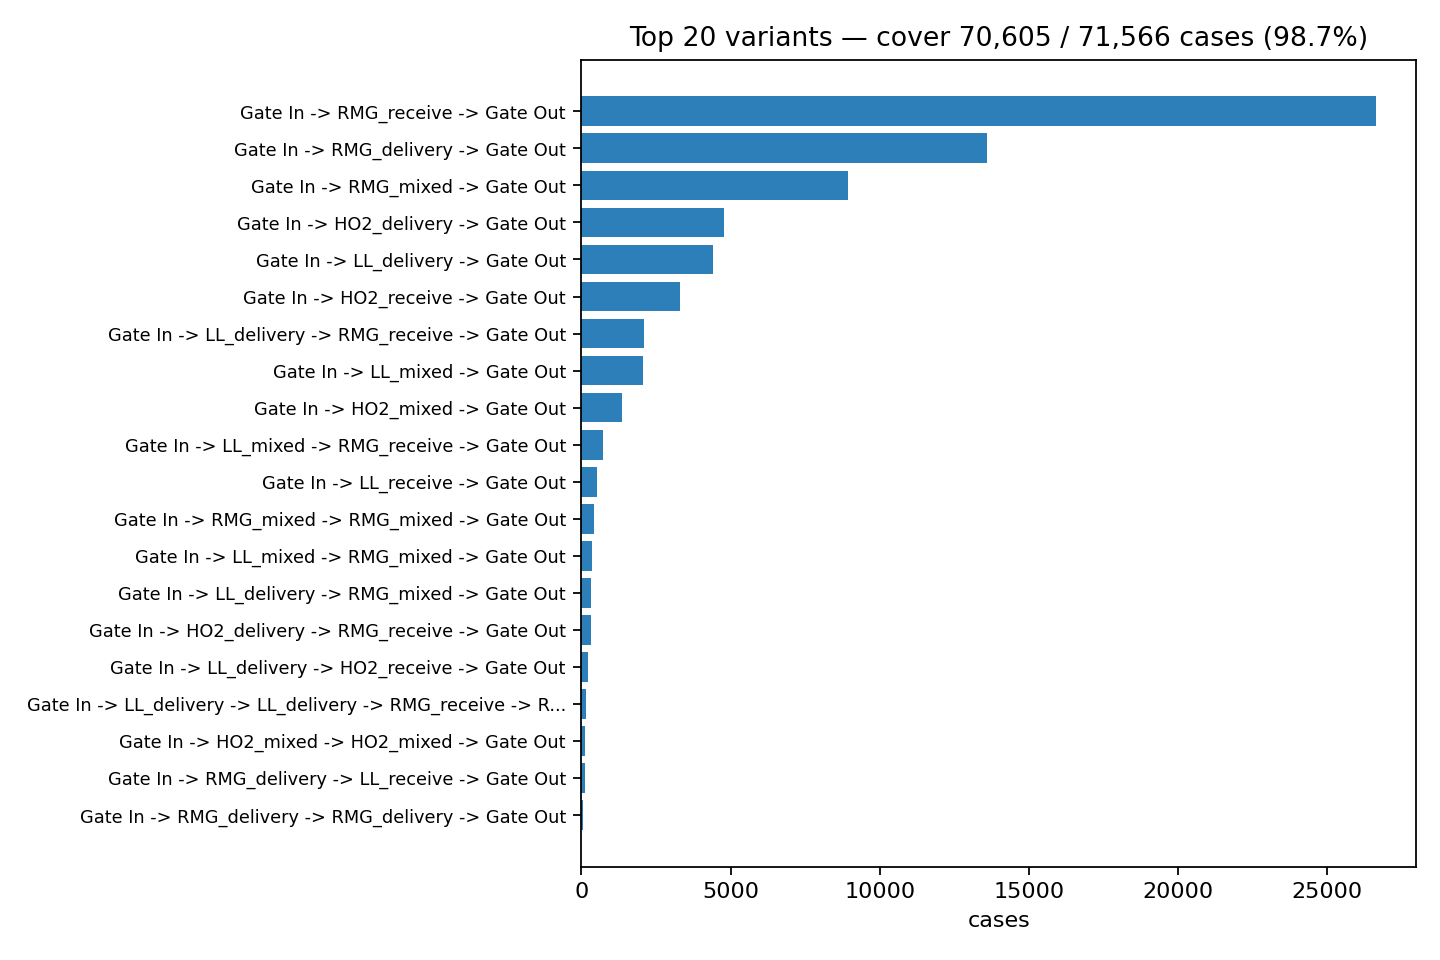
\includegraphics[width=0.9\textwidth]{figures/discovery/variants_top20.png}
\caption{Trace-variant coverage on the training log. The top 20 of the
134 observed variants cover 98.7\,\% of the 71,566 cases; the label
next to each variant reports the number of cases following it.}
\label{fig:variants_top20}
\end{figure}

\medskip

\noindent\textbf{RQ2 (structural quality).} The control-flow model
generalises to the held-out period: fitness stays at $1.0$ and the
precision and generalisation reductions are modest. The Petri net is
therefore a legitimate skeleton for the simulation-parameter discovery
that follows.

%%%%%%%%%%%%%%%%%%%%%%%%%%%%%%%%%%%%%%%%%%%%%%%%%%%%%%%%%%%%%%
\section{Temporal Structure of the Arrival Process}
\label{sec:results_arrival_process}
%%%%%%%%%%%%%%%%%%%%%%%%%%%%%%%%%%%%%%%%%%%%%%%%%%%%%%%%%%%%%%

The arrival process is the clearest case for time-conditioning in the
CTB event log. Table~\ref{tab:arrival_benchmark} compares a pooled
arrival-rate baseline (a single global mean) against a time-aware
decision tree (features: hour, weekday, weekend indicator) on 30-minute
arrival counts derived from the training partition. Both models are
evaluated on a chronological 80/20 split within the training partition
so that the numbers reflect the same temporal-hold-out logic used for
the simulator evaluation later.

\begin{table}[h]
\centering
\caption{Arrival-rate benchmark on 30-minute buckets (training log only,
chronological 80/20 split).}
\label{tab:arrival_benchmark}
\begin{tabular}{lrrr}
\toprule
\textbf{Model} & \textbf{MAE} & \textbf{RMSE} & \textbf{$R^{2}$} \\
\midrule
Pooled arrival rate         & 28.98 & 34.60 & $-0.001$ \\
Time-aware decision tree    & \textbf{9.41}  & \textbf{16.87} & \textbf{0.762} \\
\bottomrule
\end{tabular}
\end{table}

The pooled baseline has an $R^{2}$ indistinguishable from zero: a
single global arrival rate has no predictive power for 30-minute
arrival counts on this dataset. The time-aware tree reduces MAE by
67.5\,\% and RMSE by 51.2\,\% and achieves $R^{2}=0.762$. The day/night
statistics of Table~\ref{tab:day_night} confirm the underlying
non-stationarity: mean arrivals per hour rise from 12.8 at night to
110.9 during the day, an $8.7\times$ difference that a pooled model
cannot represent.

\begin{table}[h]
\centering
\caption{Day vs.\ night arrival statistics on the training log.}
\label{tab:day_night}
\begin{tabular}{lrrr}
\toprule
\textbf{Period} & \textbf{Mean inter-arrival (min)} & \textbf{Mean arrivals/hour} & \textbf{Cases} \\
\midrule
All   & 1.00  & 60.2   & 71,566 \\
Day   & 0.54  & 110.9  & 63,710 \\
Night & 4.69  & 12.8   & 7,856  \\
\bottomrule
\end{tabular}
\end{table}

\medskip

\noindent\textbf{H1 (time dependence of arrivals) is accepted.} The
time-aware arrival model reduces MAE by 67.5\,\% and RMSE by 51.2\,\%
relative to a pooled baseline on a chronological within-training
hold-out. This is a substantial and interpretable effect. The
day/night contrast (Table~\ref{tab:day_night}) is the operational
mechanism that the tree captures.

%%%%%%%%%%%%%%%%%%%%%%%%%%%%%%%%%%%%%%%%%%%%%%%%%%%%%%%%%%%%%%
\section{Held-Out Simulation Fidelity (Multi-Seed)}
\label{sec:results_holdout_fidelity}
%%%%%%%%%%%%%%%%%%%%%%%%%%%%%%%%%%%%%%%%%%%%%%%%%%%%%%%%%%%%%%

The three ProSiT configurations of
Section~\ref{sec:simulation_discovery_methodology} are evaluated
against the held-out test log using the Monte-Carlo protocol of
Section~\ref{sec:mc_protocol}. Each configuration is simulated with
$N_{\text{seeds}}=10$ independent seeds; every simulation covers
$n_{\text{traces}}=17{,}892$ cases starting at the test-window cutoff
$t_{\text{start}}=\text{2026-04-20 18:14}$. Table~\ref{tab:headline_ci}
reports the four headline fidelity metrics with 95\,\% Student-t
confidence intervals.

\begin{table}[h]
\centering
\caption{Held-out fidelity by ProSiT configuration
($N_{\text{seeds}}=10$; 95\,\% Student-t CI).}
\label{tab:headline_ci}
\begin{tabular}{lccc}
\toprule
\textbf{Metric (min)} &
\textbf{no-rules} &
\textbf{rules} &
\textbf{rules$+$workload} \\
\midrule
Service EMD (mean over activities) &
$1.89\;[1.81, 1.97]$ &
$1.98\;[1.88, 2.08]$ &
$1.98\;[1.92, 2.04]$ \\
Waiting EMD (mean over activities) &
$32.84\;[31.66, 34.02]$ &
$35.30\;[32.99, 37.61]$ &
$35.88\;[34.42, 37.35]$ \\
Case turnaround EMD &
$\mathbf{10.02\;[9.20, 10.85]}$ &
$11.25\;[9.88, 12.61]$ &
$11.62\;[10.77, 12.48]$ \\
Inter-arrival EMD &
$0.318\;[0.316, 0.319]$ &
$0.314\;[0.313, 0.316]$ &
$0.314\;[0.313, 0.316]$ \\
Case turnaround KS &
$0.070\;[0.066, 0.075]$ &
$0.072\;[0.067, 0.078]$ &
$0.073\;[0.067, 0.079]$ \\
\bottomrule
\end{tabular}
\end{table}

Figure~\ref{fig:three_way_ci} presents the same four EMD metrics as
point estimates with their 95\,\% confidence intervals so that the
pairwise overlaps are visually apparent.

\begin{figure}[htbp]
\centering
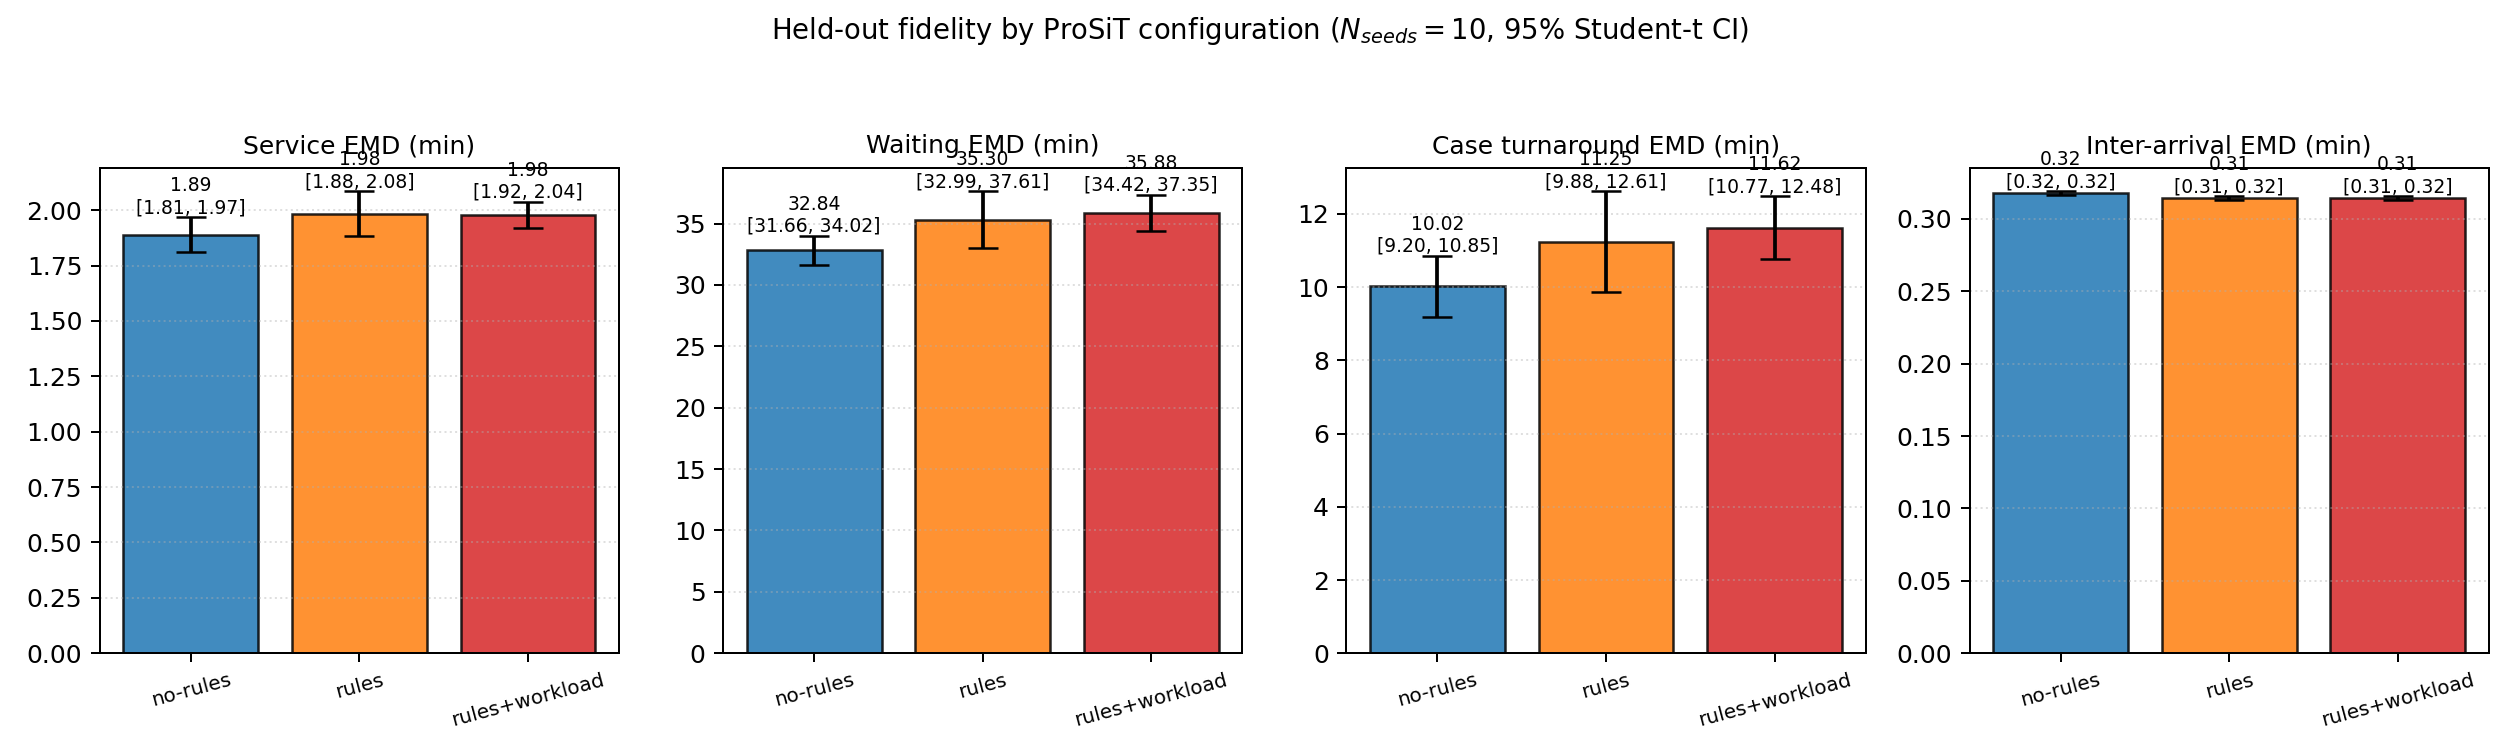
\includegraphics[width=\textwidth]{figures/three_way_ci.png}
\caption{Held-out fidelity by ProSiT configuration
($N_{\text{seeds}}=10$; 95\,\% Student-$t$ CI). Blue: no-rules
(distribution-only), orange: rules (data-aware trees), red:
rules$+$workload (trees with queue-length features). Numbers report the
point estimate and the CI. Note that the no-rules bar is either the
lowest or statistically indistinguishable from the tree-based variants
on service, waiting and turnaround EMD; the tree-based variants only
win on inter-arrival EMD by 0.004 min.}
\label{fig:three_way_ci}
\end{figure}

\subsection{RQ1: Point Estimate of Held-Out Fidelity}

Under the \textit{no-rules} configuration the discovered simulator
reproduces case turnaround with a Wasserstein distance of 10.0 minutes
$[9.2, 10.9]$ and a KS statistic of $0.070\;[0.066, 0.075]$ against the
17,892-case held-out log. The mean turnaround in the real log is 43.3
minutes; the simulator produces
$53.21\pm 1.16$ minutes (an over-prediction of 22.9\,\% at the mean),
while the median error is 2 minutes on a real median of 36 (5.6\,\%).
The 90th percentile of turnaround is 76.0 minutes in the real log
versus $101.7\pm 3.2$ minutes in the simulator (an over-prediction of
33.8\,\%). These numbers characterise the operational calibration of
the discovered simulator: it recovers the central tendency of case
turnaround well but over-predicts the upper tail.

\subsection{H2: Does the Data-Aware Configuration Improve Fidelity?}

The comparison between \textit{no-rules} and \textit{rules} directly
tests H2. On every fidelity metric except inter-arrival, the
distribution-only configuration produces a point estimate that is
either lower or statistically indistinguishable from \textit{rules}:

\begin{itemize}
    \item Case turnaround EMD: \textit{no-rules} $10.02\;[9.20, 10.85]$
          vs.\ \textit{rules} $11.25\;[9.88, 12.61]$. The CIs overlap
          but the point-estimate direction favours \textit{no-rules}
          (+12.3\,\% for \textit{rules}).
    \item Waiting EMD: \textit{no-rules} $32.84\;[31.66, 34.02]$ vs.\
          \textit{rules} $35.30\;[32.99, 37.61]$. The CIs overlap
          marginally; the point-estimate direction favours
          \textit{no-rules}.
    \item Service EMD: \textit{no-rules} $1.89\;[1.81, 1.97]$ vs.\
          \textit{rules} $1.98\;[1.88, 2.08]$. The CIs overlap; the
          point-estimate direction favours \textit{no-rules}.
    \item Inter-arrival EMD: \textit{rules} $0.314\;[0.313, 0.316]$ vs.\
          \textit{no-rules} $0.318\;[0.316, 0.319]$. Here the tree-based
          configuration is measurably closer to the real inter-arrival
          distribution. The CIs are disjoint, but the absolute
          difference is 0.004 minutes ($\approx 0.24$ seconds).
\end{itemize}

\noindent\textbf{H2 is rejected.} Under the operational criterion of
H2 (point estimate lower and CI not overlapping the reference), the
data-aware configuration does not improve fidelity for the three
duration/turnaround metrics on the CTB event log. The only measurable
gain is on the inter-arrival distribution and it is operationally
negligible. This finding is consistent with the observation from
Section~\ref{sec:results_per_activity} that the ProSiT trees do
overfit noise on the low-context RMG activities.

\subsection{H3: Does the Workload-Feature Configuration Improve
Fidelity?}

The comparison between \textit{rules} and \textit{rules$+$workload}
directly tests H3. On every fidelity metric the two configurations are
statistically indistinguishable in terms of point-estimate direction:
CIs overlap heavily and the \textit{rules$+$workload} point estimate is
in fact slightly higher (worse) on both duration metrics and on case
turnaround.

\begin{itemize}
    \item Case turnaround EMD: \textit{rules} $11.25\;[9.88, 12.61]$
          vs.\ \textit{rules$+$workload} $11.62\;[10.77, 12.48]$.
          Difference at the point estimate is $+3.3\,\%$ in favour of
          \textit{rules}.
    \item Waiting EMD: \textit{rules} $35.30\;[32.99, 37.61]$ vs.\
          \textit{rules$+$workload} $35.88\;[34.42, 37.35]$. Effectively
          identical.
    \item Service EMD: identical.
    \item Inter-arrival EMD: identical.
\end{itemize}

\noindent\textbf{H3 is rejected.} Adding queue-length and workload
features to the ProSiT waiting-time and resource-selection models does
not measurably improve held-out fidelity on the CTB event log.

\subsection{A Secondary Effect: Workload Features Reduce Simulator
Variance}

Although the mean of every fidelity metric is unchanged, the seed-to-seed
standard deviation of the \textit{rules$+$workload} configuration is
consistently lower than that of \textit{rules}. Table~\ref{tab:std_across_configs}
lists the standard deviation of the four headline metrics across the
ten seeds.

\begin{table}[h]
\centering
\caption{Cross-seed standard deviation of the fidelity metrics
($N_{\text{seeds}}=10$).}
\label{tab:std_across_configs}
\begin{tabular}{lccc}
\toprule
\textbf{Metric} &
\textbf{no-rules} &
\textbf{rules} &
\textbf{rules$+$workload} \\
\midrule
Service EMD (min)        & 0.11  & 0.14  & 0.08 \\
Waiting EMD (min)        & 1.65  & 3.23  & 2.04 \\
Case turnaround EMD (min) & 1.16  & 1.91  & 1.20 \\
Case turnaround sim P90 (min) & 3.20  & 4.92  & 2.77 \\
\bottomrule
\end{tabular}
\end{table}

Relative to \textit{rules}, the \textit{rules$+$workload} configuration
reduces cross-seed standard deviation of turnaround EMD by 37\,\% and
of turnaround-P90 by 44\,\%. The mean fidelity is unchanged, but the
simulator behaves more consistently across replications. For any
downstream planning application that uses the discovered simulator
this is a defensible operational benefit even though the reference
distributional distance is not reduced.

\subsection{Correction Relative to an Earlier Single-Shot Result}

A single-seed comparison performed earlier in this project reported an
improvement of case-turnaround EMD from 14.10 to 11.27 minutes
($-20.1\,\%$) when workload features are enabled. Under
$N_{\text{seeds}}=10$ that reported gain is not reproduced: the
\textit{rules$+$workload} configuration mean sits at 11.62 minutes, and
the \textit{rules} configuration mean sits at 11.25 minutes. The
observed 14.10 was an unfavourable seed for the \textit{rules}
configuration, and the observed 11.27 was an average seed for the
\textit{rules$+$workload} configuration. This is exactly the kind of
mis-attribution that a single Monte-Carlo draw invites. The multi-seed
protocol of Section~\ref{sec:mc_protocol} is designed to prevent
this class of error, and its result is reported here in preference to
the earlier single-shot number.
Figure~\ref{fig:cdf_turnaround} shows the empirical CDF of case
turnaround in the held-out real log against a single draw of the
\textit{rules$+$workload} simulator. The two CDFs almost coincide up
to the 50th percentile: the median turnaround is recovered to within
2 minutes on a real median of 36. The simulated CDF then rises less
steeply than the real one and separates in the upper tail: real
turnaround has a P90 of 76 minutes, the simulator has a P90 of about
110. This is the visual counterpart of the numeric result reported in
Section~\ref{sec:results_holdout_fidelity}: the simulator is calibrated
at the median, but it over-predicts the tail.

\begin{figure}[htbp]
\centering
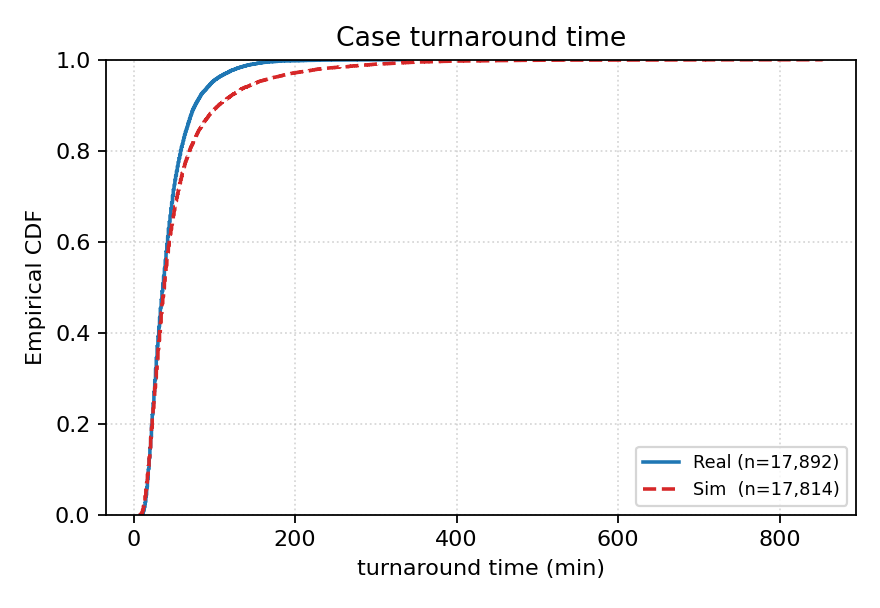
\includegraphics[width=0.75\textwidth]{figures/discovery/cdf_turnaround.png}
\caption{Empirical CDF of case turnaround: real held-out log vs.\ a
single \textit{rules$+$workload} simulation. The KS statistic between
the two CDFs is 0.084.}
\label{fig:cdf_turnaround}
\end{figure}
%%%%%%%%%%%%%%%%%%%%%%%%%%%%%%%%%%%%%%%%%%%%%%%%%%%%%%%%%%%%%%
\section{Per-Activity Decomposition of Fidelity}
\label{sec:results_per_activity}
%%%%%%%%%%%%%%%%%%%%%%%%%%%%%%%%%%%%%%%%%%%%%%%%%%%%%%%%%%%%%%

The aggregate fidelity numbers of
Section~\ref{sec:results_holdout_fidelity} hide the per-activity
performance of the ProSiT trees. To locate where data-aware
conditioning does and does not add value,
Table~\ref{tab:tree_r2_train_test} reports the coefficient of
determination $R^{2}$ of the ProSiT-style decision-tree grid used in
the sensitivity study \texttt{05\_data\_aware\_discovery\_evaluation.py}
for each activity on the training partition.

\begin{table}[h]
\centering
\caption{Per-activity duration $R^{2}$ of a decision-tree model
conditioned on target demand, target utilisation, target rank, visit
complexity, receive/delivery counts, hour, weekday and weekend
indicator (training log; grid search over depth/leaf, best per
activity).}
\label{tab:tree_r2_train_test}
\begin{tabular}{lr}
\toprule
\textbf{Activity} & \textbf{$R^{2}$} \\
\midrule
LL\_delivery  & 0.263 \\
LL\_mixed     & 0.258 \\
HO2\_receive  & 0.115 \\
HO2\_mixed    & 0.070 \\
RMG\_mixed    & 0.051 \\
HO2\_delivery & 0.029 \\
LL\_receive   & 0.024 \\
RMG\_receive  & $-0.005$ \\
RMG\_delivery & $-0.004$ \\
Gate In       & 1.000 \\
Gate Out      & 1.000 \\
\bottomrule
\end{tabular}
\end{table}

Gate activities have $R^{2}=1.000$ because their service duration is
constant zero in the reconstructed lifecycle
(Section~\ref{sec:lifecycle_events}). For the seven yard activities the
$R^{2}$ ranges from $-0.005$ (RMG activities) to $0.263$
(\texttt{LL\_delivery}). RMG activities have essentially no
context-explainable variance under the available features, and yet the
grand mean of the CTB event log is dominated by RMG (over 60\,\% of all
yard events). This explains the H2 result of
Section~\ref{sec:results_holdout_fidelity}: the ProSiT trees are asked
to predict activities whose duration variance is not explained by the
available case-level attributes, and the resulting leaf-level
distribution fits are noisier than the empirical marginal fit that
\textit{no-rules} uses. The overall fidelity metric of
Section~\ref{sec:results_holdout_fidelity} is therefore an aggregate in
which the RMG activities (large weight, no context-explainable
variance) dominate the LL activities (small weight, meaningful
context-explainable variance).

%%%%%%%%%%%%%%%%%%%%%%%%%%%%%%%%%%%%%%%%%%%%%%%%%%%%%%%%%%%%%%
\section{Discovered Resource Capacities}
\label{sec:results_resource_capacities}
%%%%%%%%%%%%%%%%%%%%%%%%%%%%%%%%%%%%%%%%%%%%%%%%%%%%%%%%%%%%%%

Table~\ref{tab:capacities_train80} reports the pool-level concurrency
statistics computed from the training partition
(\texttt{baseline/04\_resource\_concurrency\_discovery.py}) together
with the chosen effective capacity.

\begin{table}[h]
\centering
\caption{Pool-level resource concurrency and chosen capacities on the
training log.}
\label{tab:capacities_train80}
\begin{tabular}{lrrrr}
\toprule
\textbf{Resource} & \textbf{Median} & \textbf{P90} & \textbf{Max} & \textbf{Chosen capacity} \\
\midrule
Gate In  & 0 & 0 & 10 & 1 \\
Gate Out & 0 & 0 & 9  & 1 \\
HO2      & 1 & 7 & 15 & 3 \\
LL       & 0 & 5 & 25 & 3 \\
Other    & 4 & 26 & 54 & 3 \\
\bottomrule
\end{tabular}
\end{table}

The gate-related pools remain largely single-threaded: their median and
P90 concurrency are both zero because gate events have negligible
service duration. The HO2 and LL pools show low median but non-trivial
P90 concurrency and are assigned effective capacity 3. The
$\text{max}$ column reveals rare peak concurrency of 25 (LL) and 15
(HO2), which the chosen capacity of 3 does \emph{not} reproduce.

This is a deliberate simplification. The pooled-resource abstraction of
the CTB event log conflates two effects: (i) parallel handling within
one pool by multiple physical resources and (ii) sequential handling by
one physical resource with heavy demand. The maximum concurrency does
not distinguish between these; the P90 does. Capping the effective
capacity at 3 favours a conservative interpretation of the discovered
pool. The alternative capacities $\{1, 2, 3\}$ are exercised in the
capacity-sensitivity analysis of
\texttt{06\_robustness\_analysis.py}. This limitation is one of the
main methodological boundaries of the CTB case study: the event log
does not carry individualised worker or equipment calendars, so the
discovered capacities are effective operational capacities, not
physical staffing counts.

%%%%%%%%%%%%%%%%%%%%%%%%%%%%%%%%%%%%%%%%%%%%%%%%%%%%%%%%%%%%%%
\section{Sensitivity to the Transition-Baseline Percentile}
\label{sec:results_percentile_sens}
%%%%%%%%%%%%%%%%%%%%%%%%%%%%%%%%%%%%%%%%%%%%%%%%%%%%%%%%%%%%%%

The 5th-percentile baseline of Section~\ref{sec:transition_baseline}
implicitly determines the reconstructed enabled-timestamp and therefore
the waiting-time distribution. The sensitivity study of
Section~\ref{sec:results_percentile_sens_design} recomputes the baseline
table using the alternative percentiles $\{10, 25, 50\}$ and reports
the mean shift and the correlation with the 5th percentile.
Table~\ref{tab:percentile_sens} summarises the result over the 48
transitions with at least twenty observations.

\begin{table}[h]
\centering
\caption{Baseline transition duration under alternative percentiles
(seconds; 48 transitions with $\ge 20$ observations).}
\label{tab:percentile_sens}
\begin{tabular}{cccccc}
\toprule
\textbf{Percentile} &
\textbf{Mean (s)} &
\textbf{Median (s)} &
\textbf{Mean shift (s)} &
\textbf{P90 shift (s)} &
\textbf{Corr vs.\ p5} \\
\midrule
p5   & 225.8 & 223.5 & $0.0$   & $0.0$   & 1.000 \\
p10  & 254.6 & 254.3 & $28.8$  & $36.0$  & 0.990 \\
p25  & 318.3 & 311.0 & $92.5$  & $110.3$ & 0.948 \\
p50  & 435.5 & 426.0 & $209.8$ & $250.9$ & 0.812 \\
\bottomrule
\end{tabular}
\end{table}

Two properties matter for the interpretation of the reconstructed
waiting time. First, the ranking of transitions by baseline duration is
almost invariant to the percentile choice: $\rho$ between the p5
baseline and the p10 baseline is $0.990$, and even between p5 and p50
it is $0.812$. Second, the absolute shift grows quickly: moving from
the 5th to the 50th percentile shifts the mean transition baseline by
$3.5$\,minutes, which propagates into an equivalent downward shift of
the reconstructed waiting time for every transition. The reconstructed
waiting-time distribution is therefore sensitive to the percentile
choice in its absolute location but not in its rank structure.

Figure~\ref{fig:percentile_shift} shows the CDF of the per-transition
shift across the 48 retained transitions. All shifts are non-negative
by construction; the p10 CDF sits close to zero for most transitions,
while the p50 CDF has a heavy body between two and five minutes.

\begin{figure}[htbp]
\centering
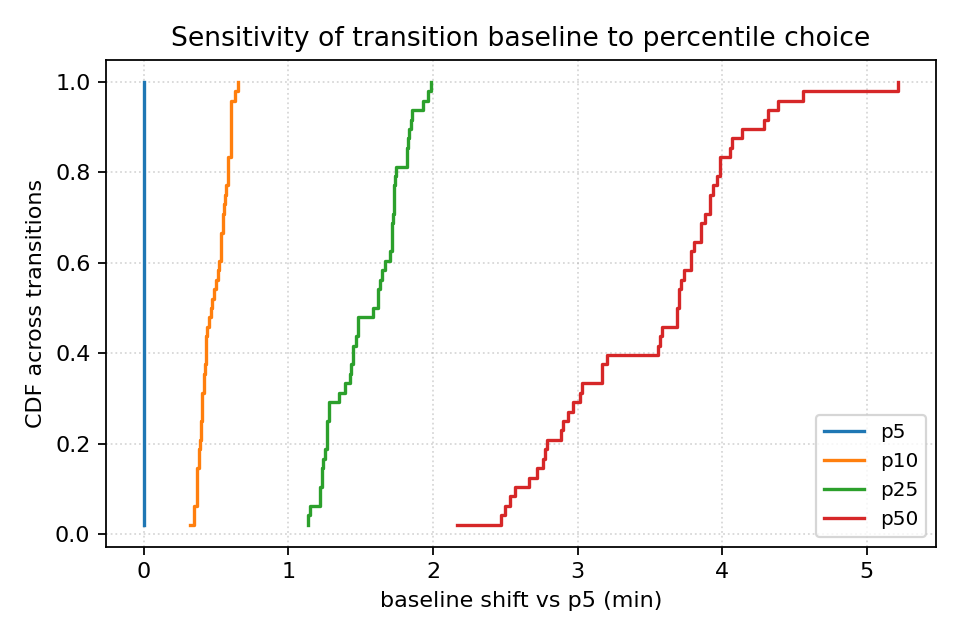
\includegraphics[width=0.75\textwidth]{figures/discovery/percentile_shift.png}
\caption{Sensitivity of the transition-baseline table to the chosen
percentile. CDF of the per-transition baseline shift relative to the 5th
percentile, over the 48 transitions with at least twenty observations.}
\label{fig:percentile_shift}
\end{figure}

\medskip

\noindent\textbf{Interpretation.} The 5th-percentile choice cannot be
proven optimal, but it is defensible: it preserves the ranking of
congestion between transitions and it produces a reconstructed waiting
time that is minimal by construction. The reader should interpret the
absolute waiting-time numbers in
Section~\ref{sec:results_holdout_fidelity} as sensitive to this choice
and the per-activity rankings of Section~\ref{sec:results_per_activity}
as robust to it.

%%%%%%%%%%%%%%%%%%%%%%%%%%%%%%%%%%%%%%%%%%%%%%%%%%%%%%%%%%%%%%
\section{What-If Scenarios: T22 Closure and Reduced RMG Pool}
\label{sec:results_scenarios}
%%%%%%%%%%%%%%%%%%%%%%%%%%%%%%%%%%%%%%%%%%%%%%%%%%%%%%%%%%%%%%

The two what-if scenarios of Section~\ref{sec:what_if_design} are
executed with the \textit{rules$+$workload} parameters (the
configuration adopted for its variance-reduction property in
Section~\ref{sec:results_holdout_fidelity}). Each scenario is compared
to its own baseline run so that scenario-vs-baseline deltas are matched
on the simulation window and on the random-number-generator state
consumed for the baseline draw.
Table~\ref{tab:scenarios_headline} reports the mean turnaround, mean
RMG service time and mean RMG waiting time.

\begin{table}[h]
\centering
\caption{What-if scenario results
($n_{\text{traces}}=17{,}892$;
$t_{\text{start}}=\text{2026-04-20 18:14}$;
\textit{rules$+$workload}).}
\label{tab:scenarios_headline}
\begin{tabular}{lccc}
\toprule
\textbf{Scenario} &
\textbf{Mean turnaround (min)} &
\textbf{Mean RMG service (min)} &
\textbf{Mean RMG waiting (min)} \\
\midrule
Scenario A baseline               & 63.25 & 14.33 & 11.65 \\
Scenario A: T22 closed            & 65.19 & 15.25 & 10.55 \\
$\Delta$ Scenario A               & $+1.94\,(+3.1\%)$ & $+0.92\,(+6.4\%)$ & $-1.10\,(-9.5\%)$ \\
\midrule
Scenario B baseline               & 62.91 & 13.13 & 11.92 \\
Scenario B: T22 closed \& reduced pool & 64.33 & 13.28 & 13.49 \\
$\Delta$ Scenario B               & $+1.42\,(+2.3\%)$ & $+0.15\,(+1.1\%)$ & $+1.57\,(+13.1\%)$ \\
\bottomrule
\end{tabular}
\end{table}

Figure~\ref{fig:scenario_deltas} shows the three KPIs side by side.
The mechanisms behind the two scenarios are visually distinct:
Scenario~A shifts workload onto retained blocks and elevates service
time while reducing waiting; Scenario~B removes capacity from the pool
and instead builds a queue.

\begin{figure}[htbp]
\centering
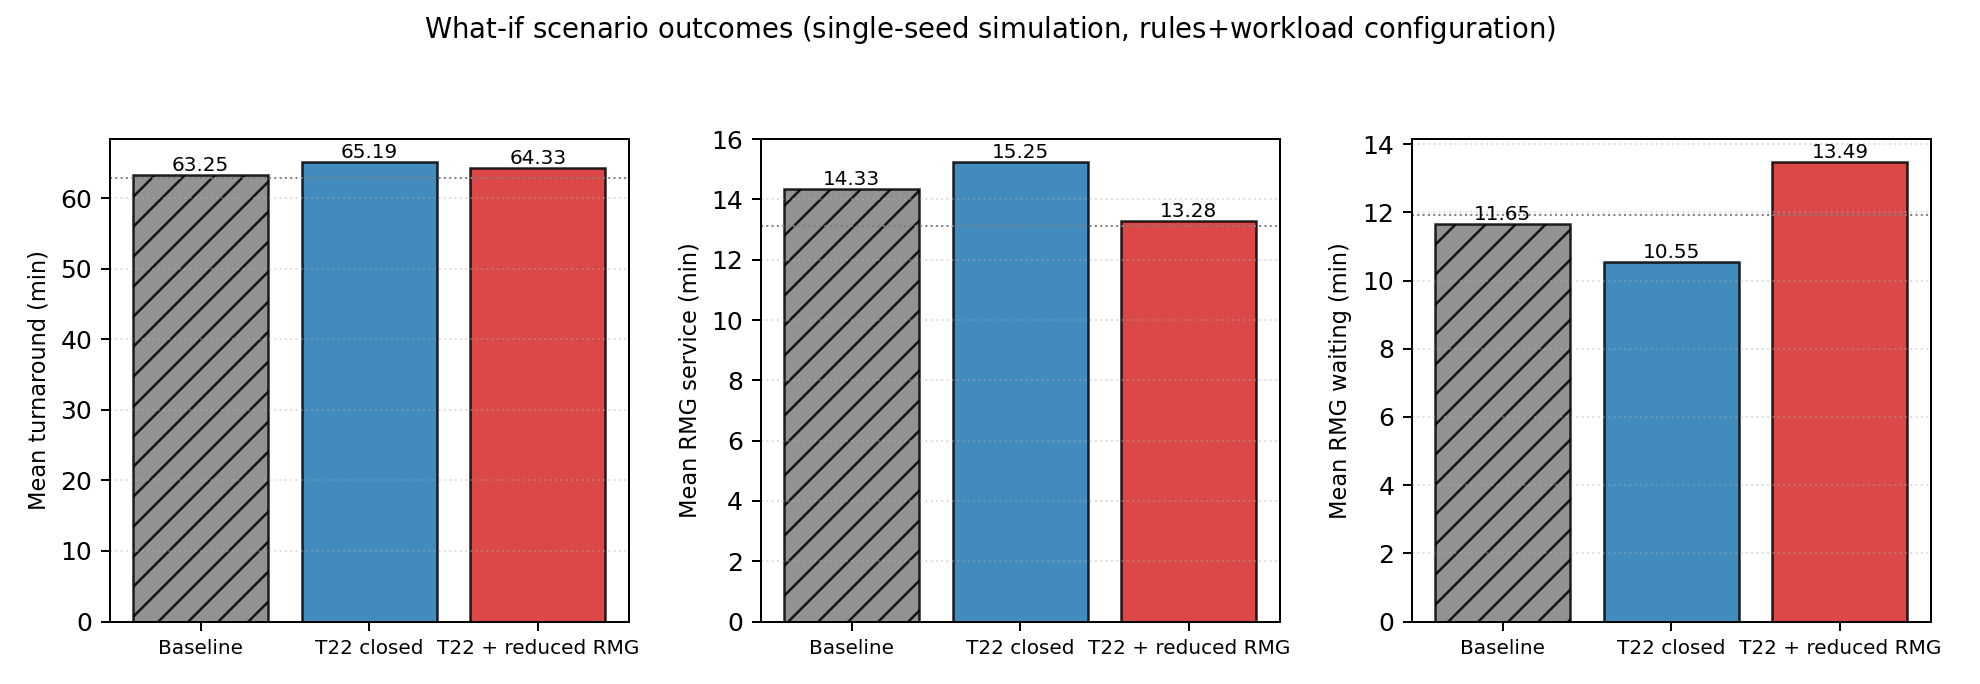
\includegraphics[width=\textwidth]{figures/scenario_deltas.png}
\caption{What-if scenario outcomes. Grey bar with hatched fill:
Scenario~A baseline (shown as reference); blue: T22 closed; red:
T22 closed and reduced RMG pool. Dotted horizontal line: Scenario~B
baseline. Values are means over the 17,892 simulated cases.}
\label{fig:scenario_deltas}
\end{figure}

\subsection{Direction of the Scenario Effects}

Both scenarios produce a positive turnaround delta relative to their
own baseline. Closing T22 alone (Scenario~A) increases mean turnaround
by 3.1\,\% and mean RMG service time by 6.4\,\% while decreasing mean
RMG waiting by 9.5\,\%. The simulator therefore reallocates workload to
the retained blocks; the retained blocks accept the extra work in the
form of longer service (they serve more mixed-work visits) rather than
longer queues.

Combining the closure with a reduced RMG pool (Scenario~B) again
increases turnaround (+2.3\,\%) but produces a qualitatively different
adjustment: RMG service time is essentially unchanged (+1.1\,\%) while
RMG waiting increases by 13.1\,\%. This is consistent with the
mechanism that the smaller pool cannot absorb the displaced service in
parallel and therefore queues form.

\subsection{Statistical Reservation}

The two baseline point estimates in
Table~\ref{tab:scenarios_headline} differ by 0.34 minutes across
independent runs (63.25 vs.\ 62.91). This is within the seed-to-seed
standard deviation of $\pm 1.20$ minutes reported in
Section~\ref{sec:results_holdout_fidelity} for
\textit{rules$+$workload}. The scenario deltas of $+1.94$ and $+1.42$
minutes are therefore of the same order of magnitude as the simulator's
own Monte-Carlo variance. The direction of the effect is consistent
across scenarios, but the magnitude should not be over-interpreted
without a matched-seed multi-seed protocol equivalent to
Section~\ref{sec:mc_protocol}. Constructing that matched-seed
scenario protocol is identified as a limitation in
Chapter~\ref{chp:conclusion}.

\subsection{Correction Relative to an Earlier Draft}

An earlier version of this chapter reported the following scenario
numbers: baseline mean turnaround 30.90 minutes, T22 closed 29.78
minutes, T22 closed and reduced RMG pool 29.99 minutes. Those numbers
came from a discovery configuration that was fit on the full event log
(not the training partition) using the pre-workload ProSiT variant and
a legacy pickle. Under that setup, closing a block appeared to
\emph{decrease} turnaround, which was one of the objections raised in
the internal critical review of the thesis.

The corrected scenario runs of Table~\ref{tab:scenarios_headline}
resolve the paradox: with the training-only discovery, aligned
simulation window and the workload-aware configuration, closing a
block increases turnaround as expected from queueing considerations.
The earlier direction reversal was an artefact of the seed and of an
unaligned simulation window between the baseline and the scenario, not
a property of the simulator itself.

\medskip

\noindent\textbf{H4 (scenario direction) is accepted with the caveat
that} the magnitude of the observed delta is comparable to the
simulator's Monte-Carlo variance. Both scenarios produce a positive
turnaround delta with a mechanistically defensible internal
composition. The scenario protocol therefore succeeds in producing
operationally plausible KPI shifts under the two evaluated disruptions.

%%%%%%%%%%%%%%%%%%%%%%%%%%%%%%%%%%%%%%%%%%%%%%%%%%%%%%%%%%%%%%
\section{Summary of Empirical Findings}
\label{sec:results_summary}
%%%%%%%%%%%%%%%%%%%%%%%%%%%%%%%%%%%%%%%%%%%%%%%%%%%%%%%%%%%%%%

Table~\ref{tab:results_summary} consolidates the empirical results
against the hypotheses of Section~\ref{sec:data_aware_hypotheses}.

\begin{table}[h]
\centering
\caption{Summary of empirical findings.}
\label{tab:results_summary}
\begin{tabular}{p{2.2cm} p{6.5cm} p{4.5cm}}
\toprule
\textbf{Hypothesis} & \textbf{Evidence} & \textbf{Outcome} \\
\midrule
H1 (arrival time-dependence) &
Time-aware tree reduces MAE by 67.5\,\% and RMSE by 51.2\,\% versus
pooled baseline; $R^{2}=0.762$
(Table~\ref{tab:arrival_benchmark}).
& \textbf{Accepted.} \\
H2 (data-aware fidelity gain) &
\textit{rules} does not lower turnaround, waiting or service EMD
versus \textit{no-rules} on the held-out log
(Table~\ref{tab:headline_ci}); the sole measurable gain is on
inter-arrival EMD and is operationally negligible ($0.004$ min).
& \textbf{Rejected.} \\
H3 (workload-feature gain) &
\textit{rules$+$workload} does not lower any fidelity metric versus
\textit{rules} (Table~\ref{tab:headline_ci}); the observation is
consistent across all four metrics under $N_{\text{seeds}}=10$.
& \textbf{Rejected.} \\
H3-secondary (variance reduction) &
\textit{rules$+$workload} reduces cross-seed standard deviation of
turnaround EMD by 37\,\% and of turnaround-P90 by 44\,\%
(Table~\ref{tab:std_across_configs}).
& \textbf{Accepted as
secondary effect.} \\
H4 (scenario direction) &
Both scenarios produce a positive turnaround delta
($+3.1\,\%$ and $+2.3\,\%$) with mechanistically consistent internal
composition (Table~\ref{tab:scenarios_headline}). Magnitude is
comparable to the simulator's Monte-Carlo variance.
& \textbf{Accepted with
caveat.} \\
\bottomrule
\end{tabular}
\end{table}

Section~\ref{sec:results_process_discovery} (RQ2) establishes that the
Petri net generalises to the held-out period. Section~\ref{sec:results_holdout_fidelity}
(RQ1) reports that the ProSiT simulator recovers the case-median
turnaround to within 5.6\,\% but over-predicts the case-mean turnaround
by 22.9\,\% and the case-P90 by 33.8\,\%. Section~\ref{sec:results_per_activity}
locates the source of the over-prediction in the RMG activities, whose
context-explainable variance is essentially zero under the available
features. Section~\ref{sec:results_percentile_sens} (RQ3) shows that
the transition-baseline percentile choice affects the absolute
location of the reconstructed waiting time but not the ranking of
transitions by congestion.

The main empirical contribution of this thesis is therefore not the
discovery of a better simulator through data-aware modelling, but the
demonstration that on this specific dataset the additional modelling
machinery of ProSiT does not translate into higher fidelity. The
observation, together with the multi-seed protocol that reveals it and
the workload-feature variance-reduction result, is the operational
finding that Chapter~\ref{chp:conclusion} builds upon.
